% The tangent line at a marked point on M_{0,n}/S_{n-1} — standalone article for Hexagon (MO 516243, folder 146).
% pdfLaTeX. Compile: latexmk -pdf article.tex (or tectonic -X compile article.tex).
\documentclass[11pt,a4paper]{amsart}
\usepackage[T1]{fontenc}
\usepackage[utf8]{inputenc}
\usepackage{lmodern,microtype,amssymb,mathtools,booktabs}
\usepackage[margin=2.7cm]{geometry}
\usepackage{tikz}
\usepackage[hidelinks]{hyperref}

\newtheorem{theorem}{Theorem}
\newtheorem{proposition}[theorem]{Proposition}
\newtheorem{lemma}[theorem]{Lemma}
\newtheorem{corollary}[theorem]{Corollary}
\theoremstyle{remark}
\newtheorem{remark}[theorem]{Remark}

\newcommand{\M}{M_{0,n}}
\newcommand{\Sn}{\mathfrak S}
\newcommand{\Pic}{\operatorname{Pic}}
\newcommand{\Aff}{\mathrm{Aff}}
\newcommand{\Gm}{\mathbb G_m}
\newcommand{\Ga}{\mathbb G_a}
\newcommand{\PP}{\mathbb P^1}
\newcommand{\disc}{\operatorname{disc}}
\newcommand{\fac}[1]{\href{https://grothendieck.umontpellier.fr/#1.pdf}{folder~#1}}

\title[The tangent line at a marked point]{The tangent line at a marked point on $M_{0,n}/\mathfrak S_{n-1}$,\\ after a table of Grothendieck}
\author{Michel Hua}
\address{Commutator, Paris, France}
\email{michel@commutator.io}
\thanks{ORCID 0009-0002-8304-0683.}
\date{7 November 2026}
\subjclass[2020]{14H10; 14C22, 14D23}
\keywords{moduli of pointed rational curves, Picard group of a quotient stack, binary forms, discriminant, tangent line bundle, Lean}

\begin{document}
\begin{abstract}
Let $L_n$ be the line bundle on $M_{0,n}$ whose fibre is the tangent line to $\mathbb P^1$ at the last marked point, and $L$ the tensor product of the tangent lines at all of them. We show that, in characteristic zero, the Picard group of the quotient stack $[M_{0,n}/\mathfrak S_{n-1}]$ is cyclic of order $(n-1)(n-2)$ for every $n \ge 3$, generated by $L_n$, and that $L$ has order $n-1$ in $\operatorname{Pic}[M_{0,n}/\mathfrak S_n]$. For even $n \ge 6$ the group was known, through the integral Chow ring computed by Edidin and Hu; the odd case does not seem to be in print. The question comes from a table in Grothendieck's working notes, which gives these orders for four points and only guesses for five and six. The proof is a few lines once the stack is written as monic squarefree polynomials modulo the affine group. An elementary version, with explicit trivialisations and fixed configurations, is formalised in Lean.
\end{abstract}

\maketitle

\section{Introduction}

Let $k$ be a field of characteristic zero and $n \ge 3$. Let $\M$ be the moduli space of $n$ distinct ordered points $x_1, \dots, x_n$ on $\PP$, up to $\mathrm{PGL}_2$. For each $i$ the tangent lines $T_{x_i}\PP$ form a line bundle $L_i$ on $\M$, and we put $L = L_1 \otimes \dots \otimes L_n$. The symmetric group $\Sn_n$ acts on $\M$ by renumbering the points and acts compatibly on $L$; the subgroup $\Sn_{n-1}$ fixing the last point acts on $L_n$. This defines classes
\[
[L] \in \Pic[\M/\Sn_n], \qquad [L_n] \in \Pic[\M/\Sn_{n-1}],
\]
and the question is their order: the least $m \ge 1$ for which $L^{\otimes m}$, or $L_n^{\otimes m}$, has a nowhere-vanishing section compatible with the action.

\begin{theorem}\label{thm:main}
For every $n \ge 3$:
\begin{enumerate}
\item $\Pic[\M/\Sn_{n-1}]$ is cyclic of order $(n-1)(n-2)$, generated by $[L_n]$;
\item $[L]$ has order $n-1$ in $\Pic[\M/\Sn_n]$.
\end{enumerate}
\end{theorem}

For $n = 4, 5, 6$ the orders are $3, 4, 5$ for $L$ and $6, 12, 20$ for $L_n$.

\subsection*{The source}
The University of Montpellier holds the mathematical papers that Alexandre Grothendieck left to Jean Malgoire, and publishes their facsimiles. Its \fac{146}, on the action of symmetric groups on $\M$, has a table on page~70 giving, for $n = 4, 5, 6$, the least exponent that makes $L$ and the $L_i$ trivial compatibly with the symmetric group. The column $n = 4$ reads $3$ for $L$ and $6$ for $L_i$, which is right. The columns $n = 5$ and $n = 6$ carry only queried values: \emph{12\,?} for both bundles when $n = 5$, and \emph{20\,?} for $L$ and \emph{60\,?} for $L_i$ when $n = 6$. Page~72 builds sections indexed by the three-element subsets of the points and concludes that $L^{\otimes 6}$ is trivial for $n = 4$ and $n = 5$. Theorem~\ref{thm:main} fills in the table: for $n = 5$ the queried $12$ is right for $L_5$ but not minimal for $L$, whose order is $4$; for $n = 6$ the orders are $5$ and $20$, not $20$ and $60$.

\begin{table}[h]\centering
\begin{tabular}{lcccccc}
\toprule
& \multicolumn{2}{c}{$n = 4$} & \multicolumn{2}{c}{$n = 5$} & \multicolumn{2}{c}{$n = 6$}\\
& $L$ & $L_n$ & $L$ & $L_n$ & $L$ & $L_n$\\
\midrule
Page 70 & 3 & 6 & 12\,? & 12\,? & 20\,? & 60\,?\\
Theorem~\ref{thm:main} & 3 & 6 & 4 & 12 & 5 & 20\\
\bottomrule
\end{tabular}
\caption{The table of \fac{146}, page~70, and the orders given by Theorem~\ref{thm:main}.}\label{tab:table}
\end{table}

\subsection*{What was known}
The stack $[\M/\Sn_n]$ is the stack of smooth binary forms of degree $n$ up to scalars. Its Picard group was computed by Arsie and Vistoli \cite{arsievistoli2004} and, for $n$ even, by Gorchinskiy and Viviani, who find $\mathbb Z/2(n-1)$ \cite[Th.~3.6]{gorchinskiyviviani2008}; the order of $[L]$ follows from their methods in a few lines, but we have not found it stated. For $n = 2g+2$ even and $g \ge 2$, Edidin and Hu compute the integral Chow ring of $[M_{0,2g+2}/\Sn_{2g+1}]$, which they present as binary forms with one marked root, as $\mathbb Z[l]/(2g(2g+1)\,l)$ \cite[Th.~1.3]{edidinhu2025}, building on Pernice's description \cite{pernice2022}; so $\Pic[\M/\Sn_{n-1}]$ is cyclic of order $(n-1)(n-2)$ for even $n \ge 6$. Their generator is the class of a character of a torus, and the identification with $L_n$ is not stated. For $n = 4$, the stack $\mathcal M_{1,1}$ is a $\mu_2$-gerbe over $[M_{0,4}/\Sn_3]$, and $\Pic \mathcal M_{1,1} = \mathbb Z/12$ \cite{mumford1965,fultonolsson2010} gives the order~$6$. For odd $n$ we found no printed statement; D.~Edidin confirms that their paper treats only the even case and that he knows no reference for the odd one \cite{edidin2026}. The question was asked on MathOverflow by the author (question 516243), with the argument of Section~\ref{sec:stack} as a self-answer.

\section{The stack as polynomials modulo the affine group}\label{sec:stack}

Put $m = n - 1 \ge 2$. Since $\mathrm{PGL}_2$ acts transitively on $\PP$, we may send the last point to $\infty$; its stabiliser is the affine group $\Aff = \Ga \rtimes \Gm$, acting on $\mathbb A^1$ by $x \mapsto ax + b$, and the other $m$ points, unordered, are the roots of a monic squarefree polynomial of degree $m$. Taking the slice $x_n = \infty$ gives an isomorphism of stacks
\[
[\M/\Sn_{n-1}] \;\cong\; [U_m/\Aff],
\]
where $U_m \subset \mathbb A^m$ is the open set of monic squarefree polynomials $x^m + c_1x^{m-1} + \dots + c_m$, on which $\Aff$ acts by substitution.

The translations $\Ga$ act freely, and every orbit meets the closed set $c_1 = 0$ exactly once, since $m$ is invertible in $k$: the translation $x \mapsto x - c_1/m$ centres the roots. So
\[
[U_m/\Aff] \;\cong\; [V_m/\Gm], \qquad V_m = \bigl\{x^m + c_2x^{m-2} + \dots + c_m \text{ squarefree}\bigr\} \subset \mathbb A^{m-1},
\]
where $\lambda \in \Gm$ acts by $x \mapsto \lambda x$, that is, on the coefficient $c_j$ with weight $j$. The complement of $V_m$ in $\mathbb A^{m-1}$ is the discriminant hypersurface $\disc = 0$. The discriminant of the generic centred polynomial is irreducible, and as a function of the roots it is $\prod_{i<j}(r_i - r_j)^2$, homogeneous of degree $m(m-1)$; so it is a semi-invariant of weight $m(m-1)$.

\begin{lemma}\label{lem:pic}
$\Pic[V_m/\Gm] \cong \mathbb Z/m(m-1)$, generated by the line bundle attached to the character $\lambda \mapsto \lambda$.
\end{lemma}

\begin{proof}
The equivariant Picard group of the affine space $\mathbb A^{m-1}$ is the character group $\mathbb Z$ of $\Gm$. Removing the irreducible divisor $\disc = 0$ gives the exact sequence
\[
\mathbb Z \cdot [\disc = 0] \longrightarrow \Pic^{\Gm}(\mathbb A^{m-1}) = \mathbb Z \longrightarrow \Pic^{\Gm}(V_m) \longrightarrow 0,
\]
and the class of the divisor of a semi-invariant of weight $w$ is the character of weight $w$, here $w = m(m-1)$.
\end{proof}

\begin{proof}[Proof of Theorem~\ref{thm:main}]
In the model $[U_m/\Aff]$ the last point is $\infty$. In the coordinate $u = 1/x$ at $\infty$, the map $x \mapsto ax + b$ is $u \mapsto u/(a + bu)$, whose derivative at $u = 0$ is $a^{-1}$; so $\Gm$ acts on $T_\infty\PP$ through the character of weight $-1$, and $[L_n]$ corresponds to $-1 \in \mathbb Z/m(m-1)$. It generates the group, which proves~(1).

At a finite root $r$, the derivative of $x \mapsto ax + b$ is $a$, so each $T_{r_i}\PP$ has weight $+1$, and the pull-back of $L$ to $[\M/\Sn_{n-1}]$ has weight $m - 1 = n - 2$. Its order in $\mathbb Z/(n-1)(n-2)$ is $n - 1$, so the order of $[L]$ is a multiple of $n - 1$. Conversely, write the points as vectors $v_i \in k^2 \smallsetminus \{0\}$ and $[v_iv_j] = \det(v_i, v_j)$. Since $T_{\langle v\rangle}\PP \cong \operatorname{Hom}(\langle v\rangle, k^2/\langle v\rangle) \cong \langle v\rangle^{\otimes -2} \otimes \det k^2$, trivialising $L^{\otimes(n-1)}$ compatibly with the action amounts to giving a nowhere-vanishing function of the $v_i$, homogeneous of degree $2(n-1)$ in each $v_i$, transforming under $g \in \mathrm{GL}_2$ by $\det(g)^{n(n-1)}$ and invariant under renumbering. The function
\[
\prod_{i \ne j}[v_iv_j] \;=\; (-1)^{n(n-1)/2}\prod_{i<j}[v_iv_j]^2
\]
is such a function: each $v_i$ occurs in $2(n-1)$ brackets, it vanishes nowhere on $\M$, and the right-hand side is invariant under $\Sn_n$. This proves~(2).
\end{proof}

\begin{remark}
For $n = 3$ the stack $[M_{0,3}/\Sn_2]$ is $B(\mathbb Z/2)$, with Picard group $\mathbb Z/2$, as the theorem says. The same computation applied to $[\M/\Sn_n]$, binary forms modulo $\mathrm{GL}_2$, recovers the results of Arsie--Vistoli and Gorchinskiy--Viviani.
\end{remark}

\section{An elementary version}

The argument can be phrased without stacks, in the vector model used above. A trivialisation of $L_n^{\otimes m}$ compatible with $\Sn_{n-1}$ is, in the same way, a nowhere-vanishing function $F(v_1, \dots, v_n)$, homogeneous of degree $2m$ in $v_n$ and $0$ in the other $v_i$, transforming by $\det(g)^m$ under $\mathrm{GL}_2$, and symmetric in $v_1, \dots, v_{n-1}$.

\emph{Upper bound.} The function
\[
F = \Bigl(\prod_{i<n}[v_iv_n]\Bigr)^{2(n-2)} \Bigm/ \prod_{\substack{i \ne j\\ i,j<n}}[v_iv_j]
\]
has these properties for $m = (n-1)(n-2)$.

\emph{Lower bound.} Let $\omega$ be a primitive $(n-1)$-th root of unity, and consider the configuration with $x_n = 0$ and $x_1, \dots, x_{n-1}$ the $(n-1)$-th roots of unity. Write $0 = \langle(0,1)\rangle$ and the other points as $\langle(z,1)\rangle$. The matrix $g = \mathrm{diag}(\omega, 1)$ fixes $(0,1)$ and permutes the vectors $(z,1)$, so $F(gv) = F(v)$ by symmetry, while $F(gv) = \det(g)^m F(v) = \omega^m F(v)$; hence $\omega^m = 1$. With $\zeta$ a primitive $(n-2)$-th root of unity and the configuration $0, \infty$ and the $(n-2)$-th roots of unity, the same argument with $\mathrm{diag}(\zeta, 1)$ gives $\zeta^m = 1$; it multiplies the vector $(1,0)$ of $\infty$ by $\zeta$, which $F$ does not see, being of degree $0$ in that variable. As $n - 1$ and $n - 2$ are coprime, $(n-1)(n-2)$ divides $m$ (Figure~\ref{fig:rot}).

\begin{figure}[ht]
\centering
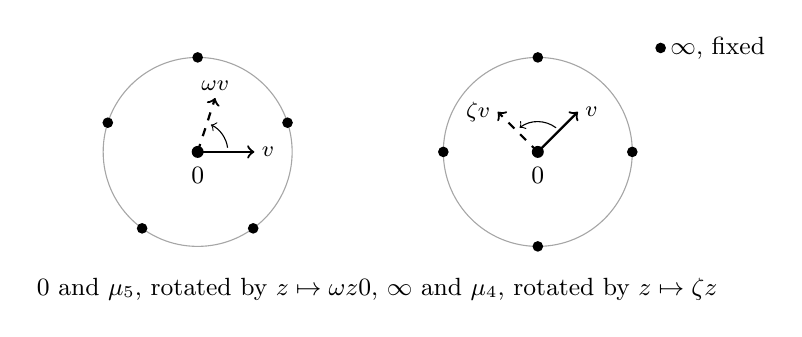
\begin{tikzpicture}[scale=1.2]
\begin{scope}
\draw[black!35] (0,0) circle (1);
\foreach \k in {0,...,4} { \fill (90+\k*72:1) circle (1.6pt); }
\fill (0,0) circle (1.8pt); \node[below=2pt] at (0,0) {\small $0$};
\draw[->,thick] (0,0) -- (0:0.6) node[right=-1pt] {\footnotesize $v$};
\draw[->,thick,dashed] (0,0) -- (72:0.6) node[above=-1pt] {\footnotesize $\omega v$};
\draw[->] (8:0.32) arc (8:64:0.32);
\node at (0,-1.45) {\small $0$ and $\mu_5$, rotated by $z \mapsto \omega z$};
\end{scope}
\begin{scope}[xshift=3.6cm]
\draw[black!35] (0,0) circle (1);
\foreach \k in {0,...,3} { \fill (\k*90:1) circle (1.6pt); }
\fill (0,0) circle (1.8pt); \node[below=2pt] at (0,0) {\small $0$};
\draw[->,thick] (0,0) -- (45:0.6) node[right=-1pt] {\footnotesize $v$};
\draw[->,thick,dashed] (0,0) -- (135:0.6) node[left=-1pt] {\footnotesize $\zeta v$};
\draw[->] (53:0.32) arc (53:127:0.32);
\fill (1.3,1.1) circle (1.6pt); \node[right] at (1.3,1.1) {\small $\infty$, fixed};
\node at (0,-1.45) {\small $0$, $\infty$ and $\mu_4$, rotated by $z \mapsto \zeta z$};
\end{scope}
\end{tikzpicture}
\caption{The two configurations of the lower bound for $n = 6$. The last point is $0$; a rotation permutes the other points and turns the tangent vector $v$ at $0$ into $\omega v$ or $\zeta v$. A trivialisation compatible with the renumbering must take the same value at both, so $5 \mid m$ and $4 \mid m$, hence $20 \mid m$ for $L_6$.}\label{fig:rot}
\end{figure}

Both directions, for every $n$, and the corresponding statements for $L$, are formalised in Lean~4 with Mathlib, over any field containing the relevant roots of unity (theorems \texttt{trivL\_iff} and \texttt{trivLi\_iff} of \texttt{Grothendieck.Folder146}, in the repositories \href{https://github.com/Commutator-IO/grothendieck-project}{Commutator-IO/grothendieck-project} and \href{https://github.com/Commutator-IO/grothendieck-project-palomar}{Commutator-IO/grothendieck-project-palomar}). What is not formalised is the dictionary between equivariant line bundles on $\M$ and such functions, that is, the identification of the equivariant Picard group with the first cohomology of $\Sn$ with values in the units; Mathlib does not have the spaces $\M$.

\section*{Statement on the use of artificial intelligence}
The transcription of folder~146, the search of the literature, the general formula, its proofs, the Lean formalisation and a first draft of this text were produced with language models (Claude Opus~5 and Opus~5.5, Anthropic), under the author's direction. The author checked the proofs and the references, and takes full responsibility for the content. The formal proofs are checked mechanically by Lean.

\section*{Acknowledgements}
The author thanks Dan Edidin for his answer about the odd case. The facsimiles are published by the University of Montpellier, \href{https://grothendieck.umontpellier.fr/}{grothendieck.umontpellier.fr}.

\begin{thebibliography}{9}
\bibitem{arsievistoli2004} A.~Arsie, A.~Vistoli, Stacks of cyclic covers of projective spaces, \emph{Compos.\ Math.} 140 (2004), 647--666, \href{https://doi.org/10.1112/S0010437X03000253}{doi:10.1112/S0010437X03000253}.
\bibitem{edidin2026} D.~Edidin, personal communication, e-mail of 28 October 2026.
\bibitem{edidinhu2025} D.~Edidin, Z.~Hu, The integral Chow rings of the stacks of hyperelliptic Weierstrass points, \emph{Michigan Math.\ J.} (2025), \href{https://doi.org/10.1307/mmj/20236479}{doi:10.1307/mmj/20236479}, arXiv:2208.00556.
\bibitem{fultonolsson2010} W.~Fulton, M.~Olsson, The Picard group of $\mathcal M_{1,1}$, \emph{Algebra Number Theory} 4 (2010), 87--104, \href{https://doi.org/10.2140/ant.2010.4.87}{doi:10.2140/ant.2010.4.87}.
\bibitem{gorchinskiyviviani2008} S.~Gorchinskiy, F.~Viviani, Picard group of moduli of hyperelliptic curves, \emph{Math.\ Z.} 258 (2008), 319--331, \href{https://doi.org/10.1007/s00209-007-0173-9}{doi:10.1007/s00209-007-0173-9}.
\bibitem{mumford1965} D.~Mumford, Picard groups of moduli problems, in \emph{Arithmetical Algebraic Geometry} (Purdue, 1963), Harper \& Row, New York, 1965, 33--81.
\bibitem{pernice2022} M.~Pernice, The integral Chow ring of the stack of 1-pointed hyperelliptic curves, \emph{Int.\ Math.\ Res.\ Not.} 2022, no.~15, 11539--11574, \href{https://doi.org/10.1093/imrn/rnab072}{doi:10.1093/imrn/rnab072}.
\end{thebibliography}

\end{document}
